% Copyright (c) 2022 by Lars Spreng
% This work is licensed under the Creative Commons Attribution 4.0 International License.

\documentclass[
11pt,notheorems,hyperref={pdfauthor=whatever}
]{beamer}

\usepackage{kotex}
\input{loadslides.tex}

\usepackage{fontspec}
\setmainhangulfont[
    Path=/Users/seojunha/Library/Fonts/,
    BoldFont=NotoSansCJKkr-Bold.otf
]{NotoSansCJKkr-Regular.otf}
\setsanshangulfont[
    Path=/Users/seojunha/Library/Fonts/,
    BoldFont=NotoSansCJKkr-Bold.otf
]{NotoSansCJKkr-Regular.otf}
\setmonohangulfont[
    Path=/Users/seojunha/Library/Fonts/,
    BoldFont=NotoSansCJKkr-Bold.otf
]{NotoSansCJKkr-Regular.otf}
\renewcommand{\familydefault}{\sfdefault}

\usepackage{tikz}
\usetikzlibrary{arrows.meta, positioning, fit, backgrounds, calc}

\addtobeamertemplate{frametitle}{}{\vspace{-0.5em}}

\newcommand{\yesmark}{\textcolor{green!45!black}{$\checkmark$}}
\newcommand{\nomark}{\textcolor{red!70!black}{$\times$}}
\newcommand{\paperbox}[2]{%
  \begin{block}{#1}
  \footnotesize #2
  \end{block}
}
\newcommand{\paperfigure}[1]{%
  \makebox[\linewidth][c]{\includegraphics[width=1.08\linewidth,height=0.58\textheight,keepaspectratio]{#1}}
}
\newcommand{\widepaperfigure}[1]{%
  \makebox[\textwidth][c]{\includegraphics[width=1.02\textwidth,height=0.55\textheight,keepaspectratio]{#1}}
}

\title[]{Related Work Survey}
\subtitle{Multimodal LLM Diagnosis + Sequential/Active Modality Acquisition}
\author[]{하서준}
\institute{DGIST}
\date{2026년 4월 23일}

\begin{document}

{
\setbeamertemplate{footline}{}
\begin{frame}
  \titlepage
\end{frame}
}
\addtocounter{framenumber}{-1}

\begin{frame}{ACTMED: Active Test Selection with LLM Simulation \hfill {\footnotesize\textcolor{gray!70}{NeurIPS 2025}}}
\centering
\widepaperfigure{figures/Actmed.png}
\vspace{0.15em}
\begin{columns}[T,onlytextwidth]
\begin{column}{0.31\textwidth}
\paperbox{핵심}{LLM을 surrogate simulator로 사용해 \textbf{BED 기반 순차 검사 선택}을 수행 \citep{estevez2025actmed}.}
\end{column}
\begin{column}{0.31\textwidth}
\paperbox{방법}{LLM이 후보 검사 결과를 여러 번 가상 샘플링하고, 각 결과가 진단 확률을 얼마나 바꾸는지 KL utility로 평가한다.}
\end{column}
\begin{column}{0.31\textwidth}
\begin{alertblock}{가져갈 점}
\scriptsize
별도 policy network 학습 없이, LLM이 \textbf{가상 검사 결과}를 만들고 utility를 계산해 다음 검사를 고르는 구조를 가져간다.
\end{alertblock}
\end{column}
\end{columns}
\end{frame}

% ----------------------------------------------------------------------------
\begin{frame}{How can images enter an LLM?}
\framesubtitle{이미지를 어떤 표현으로 바꿔 LLM에 넣는가?}
\vspace{0.2em}
\begin{columns}[T,onlytextwidth]
\begin{column}{0.48\textwidth}
\begin{tikzpicture}
\node[draw=gray!30, fill=gray!3, rounded corners=5pt, inner sep=8pt, text width=0.96\linewidth] {
\begin{minipage}{0.96\linewidth}
\Large\textbf{\textcolor{primary}{1. Text Summary}}

\vspace{0.55em}
\centering
\tikz[baseline=-0.5ex]{
\node[draw=gray!45, fill=white, rounded corners=2pt, inner sep=4pt] (img) {\scriptsize Image};
\node[draw=gray!45, fill=white, rounded corners=2pt, inner sep=4pt, right=0.42cm of img] (spec) {\scriptsize Specialist};
\node[draw=gray!45, fill=white, rounded corners=2pt, inner sep=4pt, right=0.42cm of spec] (txt) {\scriptsize Text};
\node[draw=gray!45, fill=white, rounded corners=2pt, inner sep=4pt, right=0.42cm of txt] (llm) {\scriptsize LLM};
\draw[->, thick, primary!60] (img) -- (spec);
\draw[->, thick, primary!60] (spec) -- (txt);
\draw[->, thick, primary!60] (txt) -- (llm);
}

\vspace{0.65em}
\raggedright
\footnotesize
이미지를 먼저 \textbf{진단 텍스트}로 바꾸고, 그 요약을 LLM의 \textbf{prompt input}으로 사용

\vspace{0.35em}
{\scriptsize\textcolor{gray!75}{예시: MoMA}}
\end{minipage}
};
\end{tikzpicture}
\end{column}
\begin{column}{0.48\textwidth}
\begin{tikzpicture}
\node[draw=gray!30, fill=gray!3, rounded corners=5pt, inner sep=8pt, text width=0.96\linewidth] {
\begin{minipage}{0.96\linewidth}
\Large\textbf{\textcolor{primary}{2. Visual Token}}

\vspace{0.55em}
\centering
\tikz[baseline=-0.5ex]{
\node[draw=gray!45, fill=white, rounded corners=2pt, inner sep=4pt] (img) {\scriptsize Image};
\node[draw=gray!45, fill=white, rounded corners=2pt, inner sep=4pt, right=0.35cm of img] (enc) {\scriptsize Encoder};
\node[draw=gray!45, fill=white, rounded corners=2pt, inner sep=4pt, right=0.35cm of enc] (proj) {\scriptsize Projector};
\node[draw=gray!45, fill=white, rounded corners=2pt, inner sep=4pt, right=0.35cm of proj] (llm) {\scriptsize LLM};
\draw[->, thick, primary!60] (img) -- (enc);
\draw[->, thick, primary!60] (enc) -- (proj);
\draw[->, thick, primary!60] (proj) -- (llm);
}

\vspace{0.65em}
\raggedright
\footnotesize
이미지를 vision encoder/projector가 \textbf{LLM embedding input}으로 변환해 직접 reasoning

\vspace{0.35em}
{\scriptsize\textcolor{gray!75}{예시: BLIP-2, Flamingo, LLaVA-Rad, MedTVT-R1}}
\end{minipage}
};
\end{tikzpicture}
\end{column}
\end{columns}

\vspace{0.9em}
\begin{columns}[T,onlytextwidth]
\begin{column}{0.48\textwidth}
\begin{minipage}{0.96\linewidth}
\begin{minipage}[t]{0.47\linewidth}
\fcolorbox{primary!25}{primary!3}{%
\begin{minipage}[t][4.7em][t]{0.86\linewidth}
\centering\footnotesize\textbf{장점}\\[0.25em]
투명성\\
plug-and-play\\
추가학습 없음
\end{minipage}}
\end{minipage}\hfill
\begin{minipage}[t]{0.47\linewidth}
\fcolorbox{gray!35}{gray!3}{%
\begin{minipage}[t][4.7em][t]{0.86\linewidth}
\centering\footnotesize\textbf{단점}\\[0.25em]
요약 정보 손실\\
specialist 품질 의존
\end{minipage}
}
\end{minipage}
\end{minipage}
\end{column}
\begin{column}{0.48\textwidth}
\begin{minipage}{0.96\linewidth}
\begin{minipage}[t]{0.47\linewidth}
\fcolorbox{primary!25}{primary!3}{%
\begin{minipage}[t][4.7em][t]{0.86\linewidth}
\centering\footnotesize\textbf{장점}\\[0.25em]
시각 정보 보존\\
end-to-end reasoning
\end{minipage}}
\end{minipage}\hfill
\begin{minipage}[t]{0.47\linewidth}
\fcolorbox{gray!35}{gray!3}{%
\begin{minipage}[t][4.7em][t]{0.86\linewidth}
\centering\footnotesize\textbf{단점}\\[0.25em]
학습 비용\\
연결 모듈 설계 필요
\end{minipage}
}
\end{minipage}
\end{minipage}
\end{column}
\end{columns}

\vspace{0.35em}
\begin{center}
\small
\textbf{\textcolor{primary}{방향성:}} ACTMED의 plug-and-play 장점을 살리고 중간 과정의 투명성을 가져가는 \textbf{Text Summary 기반}
\end{center}

\end{frame}

\begin{frame}{LLaVA-Rad: X-ray Image $\rightarrow$ Text Medical VLM \hfill {\footnotesize\textcolor{gray!70}{Nature Communications 2025}}}
\centering
\widepaperfigure{figures/llava_rad_overview.png}
\vspace{0.15em}
\begin{columns}[T,onlytextwidth]
\begin{column}{0.31\textwidth}
\paperbox{핵심}{흉부 X-ray를 Medical CLIP 모델과 LLM decoder로 연결해 \textbf{진단 텍스트를 생성}하는 medical foundation model \citep{wang2025llavarad}.}
\end{column}
\begin{column}{0.31\textwidth}
\paperbox{방법}{CXR $\rightarrow$ BiomedCLIP-CXR encoder $\rightarrow$ MLP projector $\rightarrow$ LLM visual token으로 연결한다.}
\end{column}
\begin{column}{0.31\textwidth}
\begin{alertblock}{가져갈 점}
\scriptsize
Modality 단위로 CXR를 acquire했을 때, X-ray 이미지를 \textbf{진단/finding 텍스트로 변환하는 specialist 모듈}로 사용할 수 있다.
\end{alertblock}
\end{column}
\end{columns}
\end{frame}

% ----------------------------------------------------------------------------
\begin{frame}{MedTVT-R1: Heterogeneous Modalities into LLM \hfill {\footnotesize\textcolor{gray!70}{arXiv 2025}}}
\centering
\widepaperfigure{figures/image copy.png}
\vspace{0.15em}
\begin{columns}[T,onlytextwidth]
\begin{column}{0.31\textwidth}
\paperbox{핵심}{ECG + CXR + LAB을 각 encoder/projector로 token화해 LLM에 넣는 \textbf{token-level multimodal fusion} 구조 \citep{zhang2025medtvt}.}
\end{column}
\begin{column}{0.31\textwidth}
\paperbox{방법}{ECG, CXR, LAB을 각각 전용 encoder로 읽고 token 형태로 바꾼 뒤, Modality Perception Layer가 어떤 modality를 더 볼지 조절하며 LLM이 최종 진단 텍스트를 생성한다.}
\end{column}
\begin{column}{0.31\textwidth}
\begin{alertblock}{가져갈 점}
\scriptsize
각 modality를 \textbf{텍스트로 변환하지 않고}, 전용 encoder/projector를 통해 \textbf{token representation으로 직접 LLM 입력에 주입하는} 개념을 참고한다.
\end{alertblock}
\end{column}
\end{columns}
\end{frame}

% ----------------------------------------------------------------------------
\begin{frame}{MoMA: Mixture-of-Multimodal-Agents \hfill {\footnotesize\textcolor{gray!70}{npj Digital Medicine 2026}}}
\centering
\makebox[\textwidth][c]{%
\begin{tikzpicture}
  \node[inner sep=0] (moma) {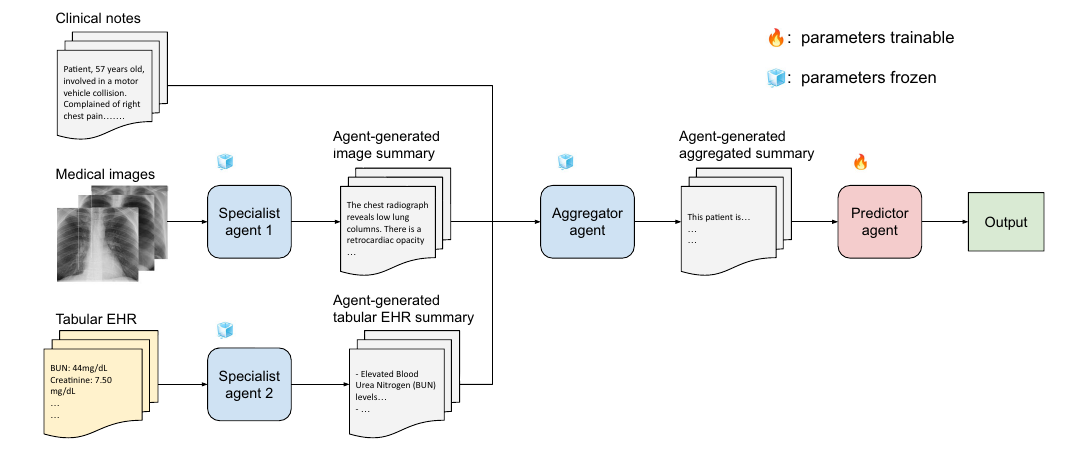
\includegraphics[width=1.02\textwidth,height=0.55\textheight,keepaspectratio]{figures/moma_architecture.png}};
  \node[anchor=south, align=center, font=\fontsize{4.6}{5}\selectfont, fill=white, fill opacity=0.9, text opacity=1, rounded corners=1pt, inner sep=1pt]
    at ($(moma.west)+(3.82,0.58)$) {CXR-LLAVA};
  \node[anchor=south, align=center, font=\fontsize{4.6}{5}\selectfont, fill=white, fill opacity=0.9, text opacity=1, rounded corners=1pt, inner sep=1pt]
    at ($(moma.west)+(3.82,-1.32)$) {Llama-3};
  \node[anchor=south, align=center, font=\fontsize{4.6}{5}\selectfont, fill=white, fill opacity=0.9, text opacity=1, rounded corners=1pt, inner sep=1pt]
    at ($(moma.west)+(9.28,0.58)$) {Llama-3};
  \node[anchor=south, align=center, font=\fontsize{4.6}{5}\selectfont, fill=white, fill opacity=0.9, text opacity=1, rounded corners=1pt, inner sep=1pt]
    at ($(moma.west)+(12.18,0.58)$) {Llama-3\\fine-tuned};
\end{tikzpicture}}
\vspace{0.15em}
\begin{columns}[T,onlytextwidth]
\begin{column}{0.31\textwidth}
\paperbox{핵심}{Specialist LLM agent가 CXR/lab을 \textbf{텍스트 요약}으로 바꾸고, aggregator/predictor가 이를 통합해 예측 \citep{gao2026moma}.}
\end{column}
\begin{column}{0.31\textwidth}
\paperbox{방법}{CXR-LLAVA와 Llama-3 specialist가 각 modality를 먼저 자연어 summary로 바꾸고, Llama-3 aggregator/predictor가 이를 통합한다.}
\end{column}
\begin{column}{0.31\textwidth}
\begin{alertblock}{가져갈 점}
\scriptsize
획득한 비텍스트 modality를 \textbf{텍스트 요약}으로 바꿔 LLM 상태에 붙이면, 학습 부담을 줄이면서 중간 과정을 사람이 검토할 수 있어 투명성을 확보할 수 있다.
\end{alertblock}
\end{column}
\end{columns}
\vspace{0.1em}
{\scriptsize \textcolor{gray!70}{Note: npj Digital Medicine volume/year 기준 2026, DOI suffix는 2025.}}
\end{frame}

% ----------------------------------------------------------------------------
\begin{frame}{Toward Our Direction: ACTMED + MoMA}
\begin{columns}[T,onlytextwidth]
\begin{column}{0.49\textwidth}
\centering
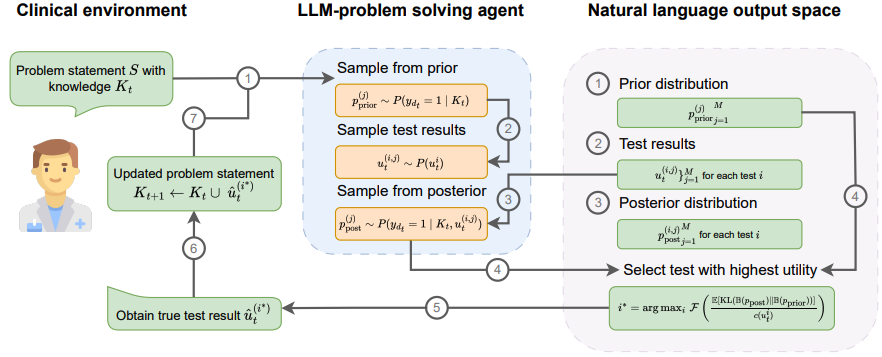
\includegraphics[width=0.98\linewidth,height=0.32\textheight,keepaspectratio]{figures/Actmed.png}
\vspace{0.25em}
\paperbox{ACTMED에서 가져갈 것}{별도 policy network를 학습하지 않고, \textbf{LLM을 surrogate}로 써서 acquisition loop를 굴리는 \textbf{추가 학습 없는 적용 가능한 설계}.}
\end{column}
\begin{column}{0.49\textwidth}
\centering
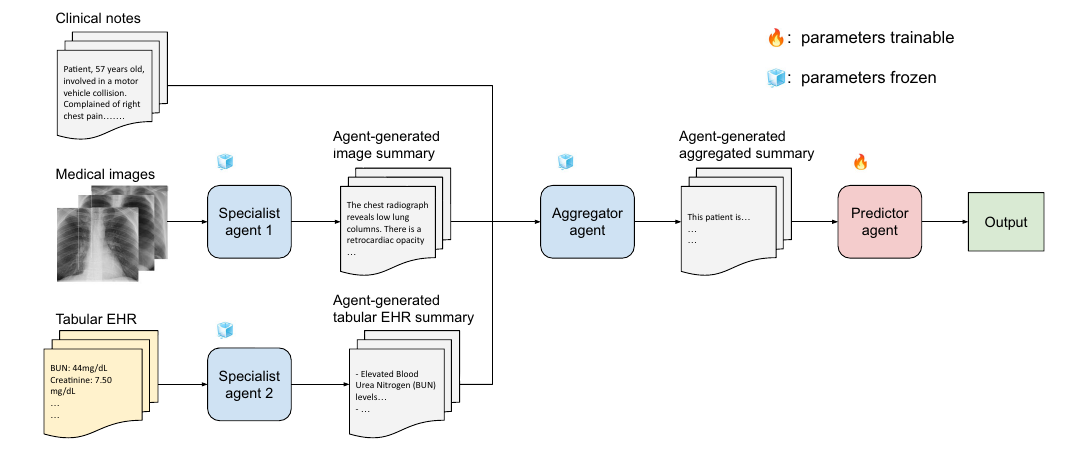
\includegraphics[width=0.98\linewidth,height=0.32\textheight,keepaspectratio]{figures/moma_architecture.png}
\vspace{0.25em}
\paperbox{MoMA에서 가져갈 것}{각 modality를 specialist가 \textbf{텍스트 요약}으로 바꾸고, 요약들을 하나의 \textbf{LLM 프롬프트로 합쳐 가는} modality-to-text abstraction 구조.}
\end{column}
\end{columns}

\vspace{0.3em}
\begin{block}{우리의 방향성}
\footnotesize
\textbf{ACTMED + MoMA}로 가면 acquisition policy는 추가 학습 없이 유지하면서, 어떤 modality든 \textbf{텍스트 요약 기반으로 투명하게} modality-level 처리할 수 있다.
\end{block}
\end{frame}

% ----------------------------------------------------------------------------
\begin{frame}{Key Challenge: Modality-level Utility Estimation}
\begin{center}
\large
\textbf{ACTMED의 BED 구조를 Modality-level로 올리면}\\
\textbf{가상 결과 simulation이 불가능해진다.}
\end{center}

\vspace{0.25em}
\begin{columns}[T,onlytextwidth]
\begin{column}{0.48\textwidth}
\begin{tikzpicture}
\node[draw=gray!65, fill=gray!8, rounded corners=3pt, inner sep=7pt, text width=0.92\linewidth] {
\begin{minipage}{0.96\linewidth}
\textbf{\textcolor{primary}{Feature-level --- ACTMED}}
\vspace{0.35em}
\scriptsize
\begin{itemize}
    \item 검사 단위: creatinine, glucose 등 수치
    \item LLM이 결과를 직접 샘플링 가능
    \item ``creatinine이 2.1 나올 것 같다''
    \item 그 결과를 더했을 때의 \textbf{posterior 확률}을 추정
    \item prior와 posterior 사이의 KL utility 계산
\end{itemize}
\end{minipage}
};
\end{tikzpicture}
\end{column}
\begin{column}{0.48\textwidth}
\begin{tikzpicture}
\node[draw=secondary, line width=0.7pt, fill=secondary!5, rounded corners=3pt, inner sep=7pt, text width=0.92\linewidth] {
\begin{minipage}{0.96\linewidth}
\textbf{\textcolor{secondary}{Modality-level --- Ours}}
\vspace{0.35em}
\scriptsize
\begin{itemize}
    \item 검사 단위: CXR / ECG / Lab panel
    \item CXR $\rightarrow$ 이미지 생성 불가
    \item ECG $\rightarrow$ 파형 생성 불가
    \item output space가 달라 동일한 simulation 불성립
\end{itemize}
\end{minipage}
};
\end{tikzpicture}
\end{column}
\end{columns}

\vspace{0.25em}
\begin{tikzpicture}
\node[draw=orange!80!black, fill=orange!8, rounded corners=3pt, inner sep=5pt, text width=0.93\textwidth] {
\begin{minipage}{0.97\linewidth}
\textbf{\textcolor{orange!80!black}{Unguided Text Simulation의 신뢰성}}

\vspace{0.2em}

\scriptsize
현재 환자 정보만 주고 LLM이 미획득 modality 소견을 바로 생성하게 하면,
실제 modality outcome distribution과 달라져 simulation 품질이 크게 떨어질 수 있다.
\end{minipage}
};
\end{tikzpicture}

\vspace{0.25em}
\begin{tikzpicture}
\node[draw=tertiary!80!black, fill=tertiary!8, rounded corners=3pt, inner sep=6pt, text width=0.93\textwidth] {
\begin{minipage}{0.97\linewidth}
\textbf{\textcolor{tertiary}{해결책: RAG-grounded Finding Scenario Generation}}
\vspace{0.2em}
\scriptsize
\begin{itemize}
    \item raw modality 자체가 아니라 finding 텍스트를 생성하되, 유사 환자의 실제 임상 소견을 RAG로 검색해 prompt context로 제공
    \item 예: 현재 검사 결과 + ECG 파형이 비슷한 환자를 찾고, 그들의 CXR 소견을 참고
    \item LLM이 이를 참고해 ``해당 modality를 찍었을 때 나올 법한 finding 텍스트''를 N개 생성
    \item 생성된 finding scenario마다 posterior를 추정하고 Expected KL로 utility 계산
\end{itemize}
\vspace{-0.25em}
{\fontsize{6.8}{7.4}\selectfont\textcolor{tertiary!70!black}{유사 환자의 실제 소견으로 grounding해 LLM 생성 결과가 임상적으로 비현실적인 방향으로 벗어나는 것을 억제할 수 있다 (hallucination 억제).}}

\vspace{0.12em}
{\fontsize{6.8}{7.4}\selectfont\textcolor{red!75!black}{유사 환자 정보에 과도하게 치우치지 않도록 prompt/모듈 설계가 필요하며, 실제 성능 향상 여부는 실험으로 검증해야 한다.}}
\end{minipage}
};
\end{tikzpicture}
\end{frame}

\begin{frame}{Our Proposed Model}
\centering
\begin{block}{핵심 아이디어}
\scriptsize
각 modality를 진단 텍스트로 요약해 aggregator agent가 융합하고, 벡터 DB의 유사 환자를 참고해 가상 결과 텍스트를 생성한 뒤 posterior utility로 다음 modality를 선택한다.
\end{block}
\vspace{0.45em}
\makebox[\textwidth][c]{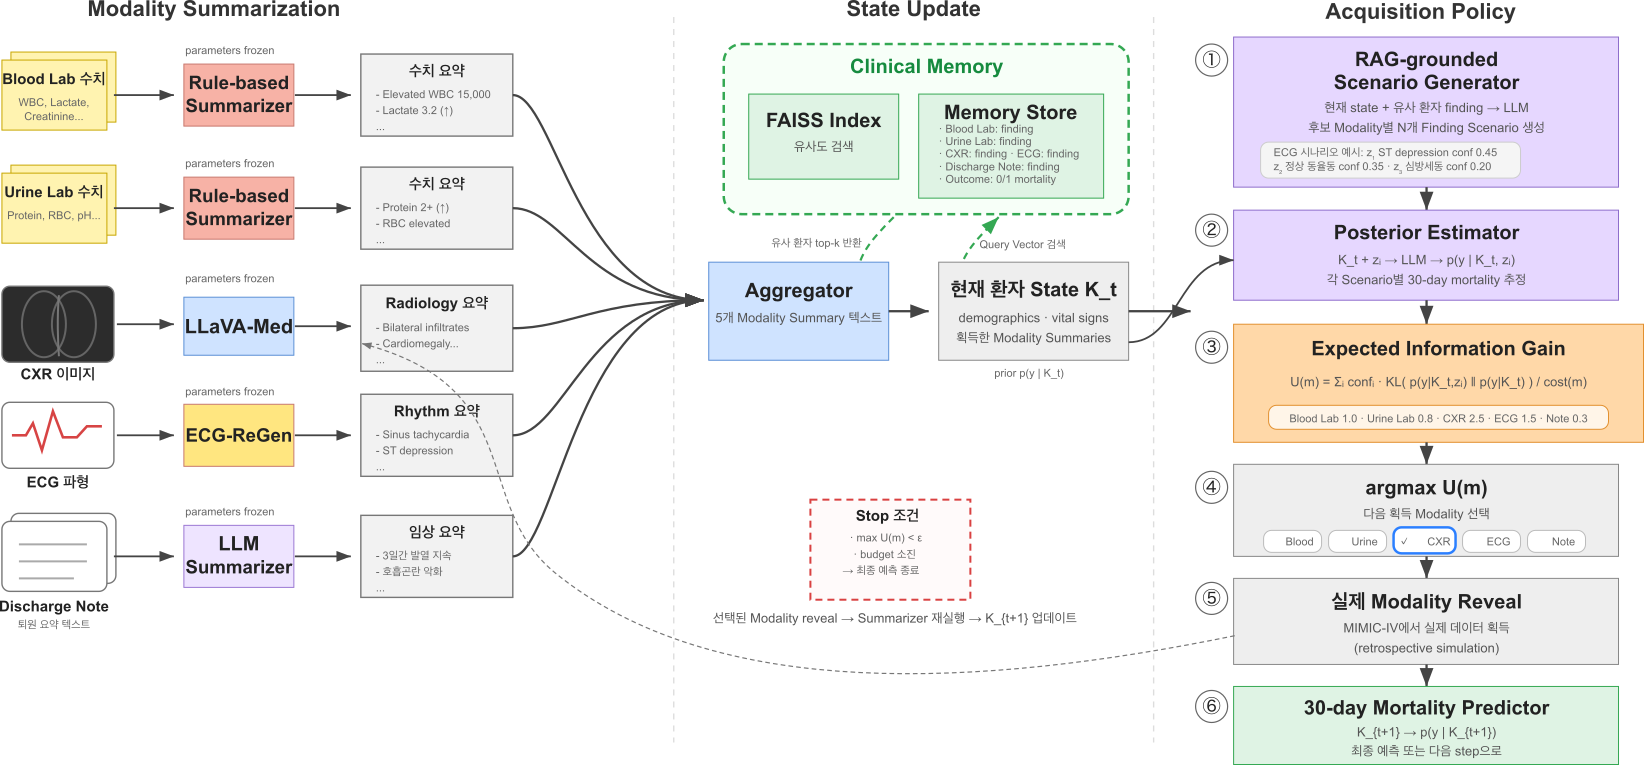
\includegraphics[width=0.955\paperwidth,height=0.70\textheight,keepaspectratio]{figures/model.png}}
\end{frame}

% ----------------------------------------------------------------------------
\begin{frame}[fragile]{Prompt Comparison: ACTMED vs. Ours}
\begin{columns}[T,onlytextwidth]
\begin{column}{0.48\textwidth}
\begin{block}{ACTMED: Feature-level Sampling}
\scriptsize
\begin{tikzpicture}
\node[draw=gray!55, fill=gray!6, rounded corners=2pt, inner sep=5pt, text width=0.94\linewidth] {
\begin{minipage}{0.96\linewidth}
\textbf{Prompt 예시 (CKD lab test)}\\
당신은 신장내과 전문의입니다. 현재 환자 정보와 병력을 바탕으로
\textbf{\$feature\_to\_sample}의 임상적으로 가능한 값을 무작위로 하나 생성하세요.
평균값만 반환하지 말고, plausible range 안에서 전형값, edge case, outlier를 반영하세요.

\vspace{0.25em}
반환값은 Python float으로 parse 가능한 \textbf{숫자 하나}여야 하며, 단위나 설명은 쓰지 마세요.

\vspace{0.2em}
\textbf{Input}\\[-0.8em]
\begin{verbatim}
Known: age 63, poor appetite,
edema, hypertension, ...
Target feature: serum creatinine
\end{verbatim}
\vspace{-1.1em}
\textbf{Output}\\[-0.8em]
\begin{verbatim}
2.7
\end{verbatim}
\end{minipage}
};
\end{tikzpicture}
\vspace{0.1em}
{\tiny\textcolor{primary}{이 sampling prompt를 $M=10$번 반복하고, 각 sample의 posterior KL을 평균낸다.}}
\end{block}
\end{column}

\begin{column}{0.48\textwidth}
\begin{alertblock}{Ours: Modality-level Scenario Sampling}
\scriptsize
\begin{tikzpicture}
\node[draw=secondary!55, fill=secondary!4, rounded corners=2pt, inner sep=5pt, text width=0.94\linewidth] {
\begin{minipage}{0.96\linewidth}
\textbf{Prompt 예시 (CXR scenario)}\\
당신은 중환자의학 전문의입니다. 현재 환자 state $K_t$와 RAG로 검색된 유사 환자들의 임상 소견을 참고해,
아직 obtain하지 않은 \textbf{CXR modality}에서 나올 법한 finding scenario를 생성하세요.
유사 환자 값을 그대로 복사하지 말고, 현재 환자에 맞는 가능한 소견을 생성하세요.

\vspace{0.25em}
각 scenario는 finding 텍스트와 confidence (0--1)를 포함하세요. confidence는 이 소견이 현재 환자에게 실제로 나타날 가능성을 의미합니다.

\vspace{0.2em}
\textbf{Input}\\[-0.8em]
\begin{verbatim}
Known: age 68, BP 92/58,
Blood lab: WBC 15000, lactate 3.2
Retrieved: similar ECG/lab cases
\end{verbatim}
\vspace{-1.1em}
\textbf{Output}\\[-0.8em]
\begin{verbatim}
{"finding": "bilateral infiltrates",
 "confidence": 0.82}
\end{verbatim}
\end{minipage}
};
\end{tikzpicture}
\vspace{0.1em}
{\tiny\textcolor{secondary}{이 prompt를 $N$번 반복해 scenario set을 만들고, confidence를 scaling한 뒤 posterior KL을 가중합한다.}}
\end{alertblock}
\end{column}
\end{columns}

\vspace{0.2em}
\begin{columns}[T,onlytextwidth]
\begin{column}{0.48\textwidth}
\centering
\scriptsize
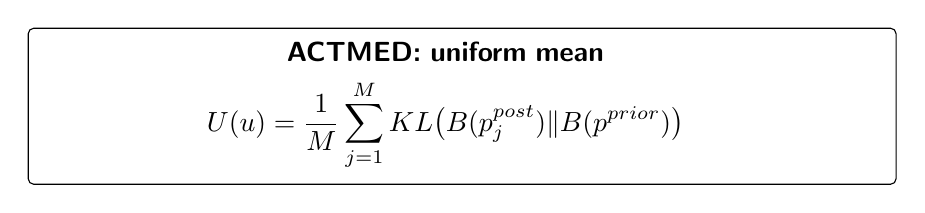
\begin{tikzpicture}
\node[draw=black, fill=white, rounded corners=2pt, inner sep=5pt, text width=0.88\linewidth] {
\begin{minipage}{0.96\linewidth}
\centering
\textbf{ACTMED: uniform mean}\\[-0.4em]
\[
U(u)=\frac{1}{M}\sum_{j=1}^{M}
KL\!\left(B(p_j^{post})\Vert B(p^{prior})\right)
\]
\end{minipage}
};
\end{tikzpicture}
\vspace{0.1em}
\parbox{0.88\linewidth}{\raggedright\fontsize{6.8}{7.4}\selectfont\textcolor{red!75!black}{분포의 tail에 있는 sample도 평균에서 같은 중요도로 반영될 수 있다.}}
\end{column}
\begin{column}{0.48\textwidth}
\centering
\scriptsize

\begin{tikzpicture}
\node[draw=black, fill=white, rounded corners=2pt, inner sep=5pt, text width=0.88\linewidth] {
\begin{minipage}{0.96\linewidth}
\centering
\textbf{Ours: adaptive weighting}\\[-0.4em]
\[
U(m)=\sum_i \tilde w_i\,
KL\!\left(B(p_i^{post})\Vert B(p^{prior})\right)
\]
\end{minipage}
};
\end{tikzpicture}
\vspace{0.1em}
\parbox{0.88\linewidth}{\raggedright\fontsize{6.8}{7.4}\selectfont\textcolor{tertiary!70!black}{분포 중심에 가까운 reliable scenario는 confidence를 높이고, 바깥쪽 scenario는 낮게 반영한다.}}
\end{column}
\end{columns}
\end{frame}

% ----------------------------------------------------------------------------
\begin{frame}{References}
\scriptsize
\printbibliography
\end{frame}

\end{document}
